

%%%%%%%%%%%%%%%%%%%%%%%%%%%%%%%%%%%%%%%%%%%%%%%%%%%%%%%%%%%%%%%%%%%%%%%%%%%%%%%%%%
\begin{frame}[fragile]\frametitle{}
\begin{center}
{\Large Conclusions}
\end{center}
\end{frame}

%%%%%%%%%%%%%%%%%%%%%%%%%%%%%%%%%%%%%%%%%%%%%%%%%%%%%%%%%%%
\begin{frame}[fragile]\frametitle{Limitations}


\begin{itemize}
\item Size of the language models: GPT index - https://github.com/jerryjliu/gpt\_index
\item Memory \& sequence of calls: LangChain - https://github.com/hwchase17/langchain
\item Correctness of the output, ChatGPT Hallucinations
\end{itemize}	 

Boie is a real company, the product name is not real. So, see what you get \ldots

\begin{lstlisting}
prompt = f"""
Tell me about AeroGlide UltraSlim Smart Toothbrush by Boie
"""
response = get_completion(prompt)
print(response)
\end{lstlisting}	 
		
\end{frame}



%%%%%%%%%%%%%%%%%%%%%%%%%%%%%%%%%%%%%%%%%%%%%%%%%%%%%%%%%%%
\begin{frame}[fragile]\frametitle{New Roles?}

Coming up with good prompt is a combination of art and science

\begin{center}
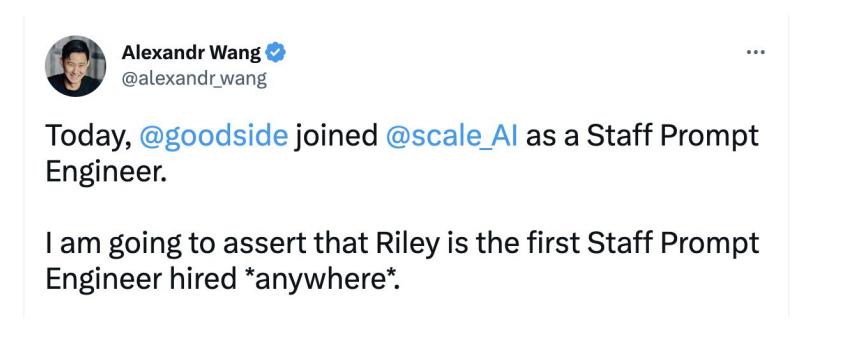
\includegraphics[width=0.8\linewidth,keepaspectratio]{promptengg5}

{\tiny (Ref: Prompt Engineering Sudalai Rajkumar)}

\end{center}		
		


\end{frame}

%%%%%%%%%%%%%%%%%%%%%%%%%%%%%%%%%%%%%%%%%%%%%%%%%%%%%%%%%%%

\begin{frame}[fragile]\frametitle{Read on to learn how to engineer good prompts!}

\begin{itemize}
\item Shin, T., Razeghi, Y., Logan IV, R. L., Wallace, E., \& Singh, S. (2020). AutoPrompt: Eliciting Knowledge from Language Models with Automatically Generated Prompts. Proceedings of the 2020 Conference on Empirical Methods in Natural Language Processing (EMNLP). https://doi.org/10.18653/v1/2020.emnlp-main.346 
\item Kojima, T., Gu, S. S., Reid, M., Matsuo, Y., \& Iwasawa, Y. (2022). Large Language Models are Zero-Shot Reasoners. 
\item Liu, P., Yuan, W., Fu, J., Jiang, Z., Hayashi, H., \& Neubig, G. (2022). Pre-train, Prompt, and Predict: A Systematic Survey of Prompting Methods in Natural Language Processing. ACM Computing Surveys. https://doi.org/10.1145/3560815 
\item Brown, T. B., Mann, B., Ryder, N., Subbiah, M., Kaplan, J., Dhariwal, P., Neelakantan, A., Shyam, P., Sastry, G., Askell, A., Agarwal, S., Herbert-Voss, A., Krueger, G., Henighan, T., Child, R., Ramesh, A., Ziegler, D. M., Wu, J., Winter, C., … Amodei, D. (2020). Language Models are Few-Shot Learners. 
\item Zhao, T. Z., Wallace, E., Feng, S., Klein, D., \& Singh, S. (2021). Calibrate Before Use: Improving Few-Shot Performance of Language Models.
\end{itemize}
\end{frame}



%%%%%%%%%%%%%%%%%%%%%%%%%%%%%%%%%%%%%%%%%%%%%%%%%%%%%%%%%%%
\begin{frame}[fragile]\frametitle{My Sketchnote}

\begin{center}
\includegraphics[width=0.45\linewidth,keepaspectratio]{PromptEng_Sketchnote_Medium}

{\tiny (Ref: https://medium.com/technology-hits/prompting-is-all-you-need-5dddb82bd022)}
\end{center}		

\end{frame}

%%%%%%%%%%%%%%%%%%%%%%%%%%%%%%%%%%%%%%%%%%%%%%%%%%%%%%%%%%%%%%%%%%%%%%%%%%%%%%%%%%
\begin{frame}[fragile]\frametitle{Resources}
\begin{itemize}
\item Prompt Engineering Guide https://github.com/dair-ai/Prompt-Engineering-Guide
\item Awesome ChatGPT Prompts https://github.com/f/awesome-chatgpt-prompts/
\item ChatGPT Prompt Engineering for DevelopersChatGPT Prompt Engineering for Developers - Deep Learning AI
\end{itemize}	 
\end{frame}

